\chapter{Similariteit}

Een similariteitsmaat voor afbeeldingen is een maat die de gelijkenis tussen twee gegeven
afbeelding uitdrukt als een getal uit het interval $[0,1]$. Dit getal nadert naar 1
naarmate de gelijkenis groter is. Bijgevolg kunnen we een dergelijke maat gebruiken om
een lijst van zoekresultaten te herordenen volgens similariteit met een bepaalde 
voorbeeld-afbeelding uit die lijst. 

We construeren een similariteitsmaat voor afbeeldingen in twee stappen. Eerst identificeren we
een afbeelding, al dan niet rechtstreeks, met een (L-)vaagverzameling. Daarna maken we gebruik van
de vaagsimilariteitsmaten uit \ref{sectie:vaagsimilariteitsmaten} om deze (L-)vaagverzamelingen te
vergelijken. 

In het vervolg van deze scriptie bedoelen we met de term ``similariteitsmaat'' steeds
een similariteitsmaat voor afbeeldingen. Dit omvat dus zowel een manier van identificeren als een 
vaagsimilariteitsmaat.

\section{Eigenschappen}

In dit hoofdstuk constueren we een aantal similariteitsmaten voor afbeeldingen. Hierbij eisen we  
dat al onze similariteitsmaten \emph{reflexief} en \emph{symmetrisch} zijn.

\subsection{Reflexiviteit}

Voor twee identieke beelden verwachten we dat een similariteitsmaat $M$ als output $1$
teruggeeft. Met andere woorden, voor een beeld $A$ moet gelden: $M(A,A)=1$.
Deze eigenschap heeft als gevolg dat de voorbeeld-afbeelding zich steeds vooraan in
de geordende lijst van zoekresultaten moet bevinden.

\subsection{Symmetrisch}

De output van een similariteitsmaat $M$ wordt verwacht onafhankelijk te zijn van de 
volgorde waarin de beelden aangeboden worden. Voor beelden $A$ en $B$ moet dus gelden:
$M(A,B)=M(B,A)$.

\section{Evaluatie van performantie}

\subsection{Globale genormaliseerde gemiddelde rang (GGGR)}

Om uit meerdere similariteitsmaten de meest geschikte te kiezen, 
moeten we een manier vinden om een dergelijke maat objectief te beoordelen. 
Dit zullen we doen door elke
maat, voor een bepaalde voorbeeld-afbeelding, toe te passen op een eenzelfde collectie 
van afbeeldingen. Vervolgens zullen we de rangschikking die we zo bekomen
beoordelen met behulp van een performantiemaat.

Figuur~\ref{fig:testcollectie} bevat de collectie van afbeeldingen die we gaan 
gebruiken. Deze collectie bestaat uit een selectie van beelden uit
de \emph{Columbia object image library} \cite{coil-100}. Deze bibliotheek van afbeeldingen 
werd gegenereerd 
door een aantal roterende objecten op bepaalde vaste momenten te fotograferen. 
Onze testcollectie bestaat uit foto's van elf objecten. Van elke object zijn
er zes momentopnames, wat een totaal van $11 \cdot 6 = 66$ afbeeldingen geeft.

\begin{figure}[p]
\begin{center}

\begin{tabular}{cccccc}

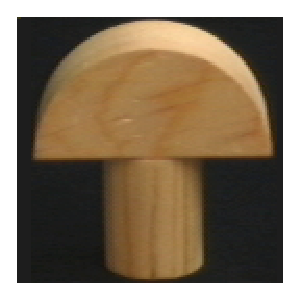
\includegraphics[width=2cm]{coil/beeld-0.eps} &
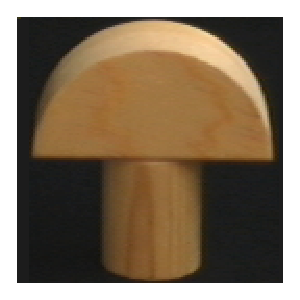
\includegraphics[width=2cm]{coil/beeld-1.eps} &
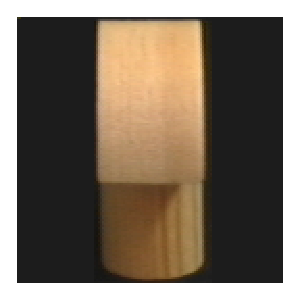
\includegraphics[width=2cm]{coil/beeld-2.eps} &
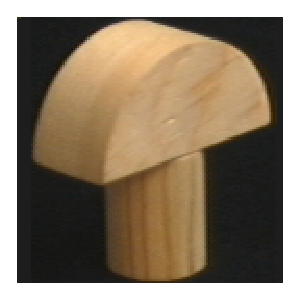
\includegraphics[width=2cm]{coil/beeld-3.eps} &
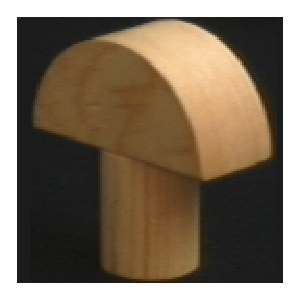
\includegraphics[width=2cm]{coil/beeld-4.eps} &
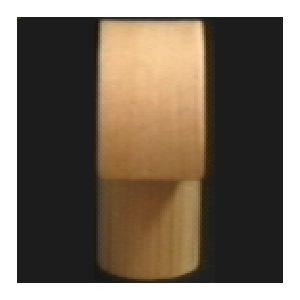
\includegraphics[width=2cm]{coil/beeld-5.eps} \\

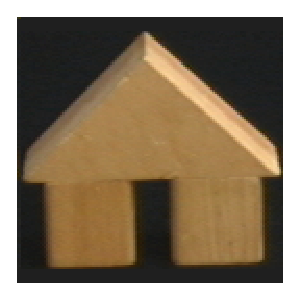
\includegraphics[width=2cm]{coil/beeld-42.eps} &
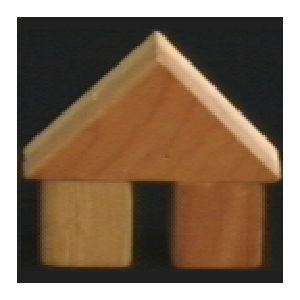
\includegraphics[width=2cm]{coil/beeld-43.eps} &
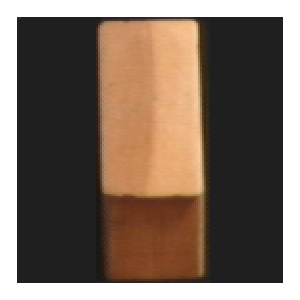
\includegraphics[width=2cm]{coil/beeld-44.eps} &
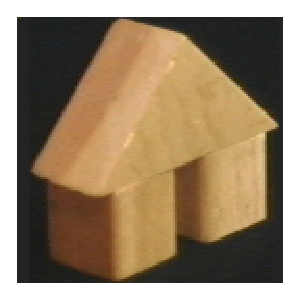
\includegraphics[width=2cm]{coil/beeld-45.eps} &
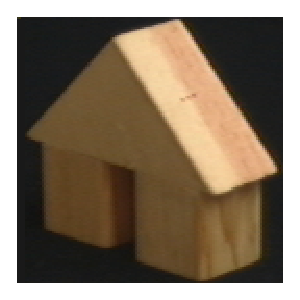
\includegraphics[width=2cm]{coil/beeld-46.eps} &
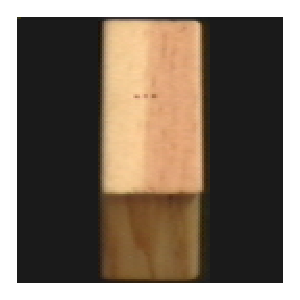
\includegraphics[width=2cm]{coil/beeld-47.eps} \\

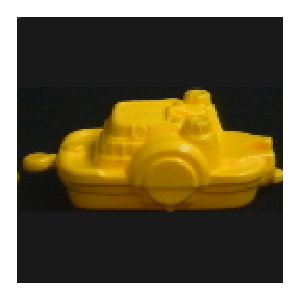
\includegraphics[width=2cm]{coil/beeld-12.eps} &
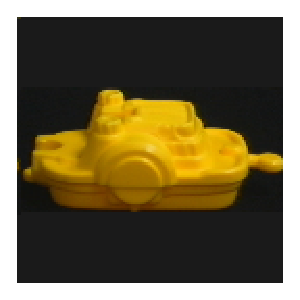
\includegraphics[width=2cm]{coil/beeld-13.eps} &
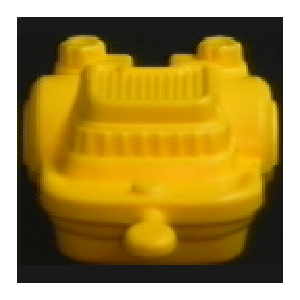
\includegraphics[width=2cm]{coil/beeld-14.eps} &
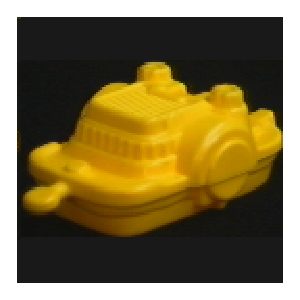
\includegraphics[width=2cm]{coil/beeld-15.eps} &
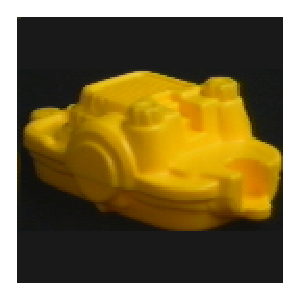
\includegraphics[width=2cm]{coil/beeld-16.eps} &
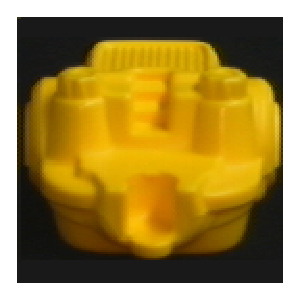
\includegraphics[width=2cm]{coil/beeld-17.eps} \\

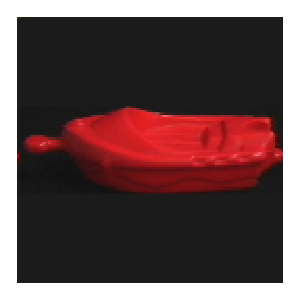
\includegraphics[width=2cm]{coil/beeld-18.eps} &
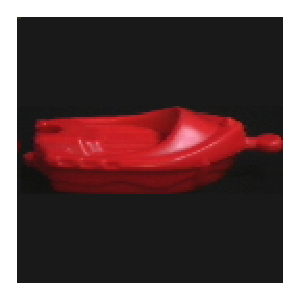
\includegraphics[width=2cm]{coil/beeld-19.eps} &
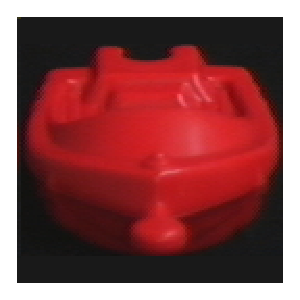
\includegraphics[width=2cm]{coil/beeld-20.eps} &
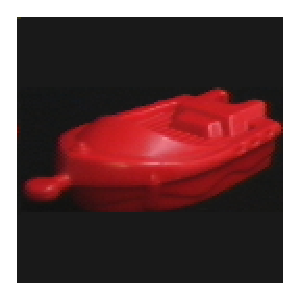
\includegraphics[width=2cm]{coil/beeld-21.eps} &
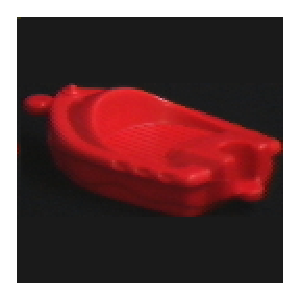
\includegraphics[width=2cm]{coil/beeld-22.eps} &
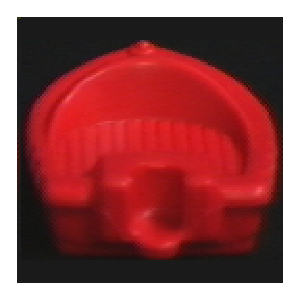
\includegraphics[width=2cm]{coil/beeld-23.eps} \\

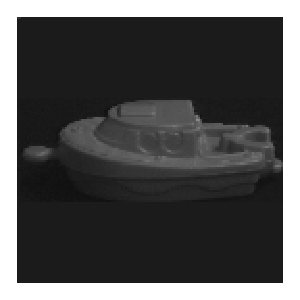
\includegraphics[width=2cm]{coil/beeld-24.eps} &
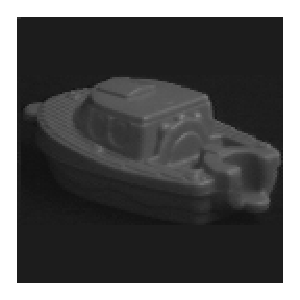
\includegraphics[width=2cm]{coil/beeld-25.eps} &
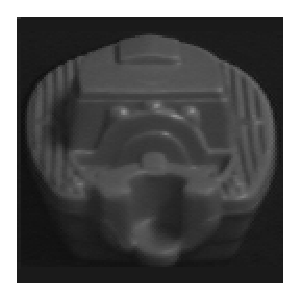
\includegraphics[width=2cm]{coil/beeld-26.eps} &
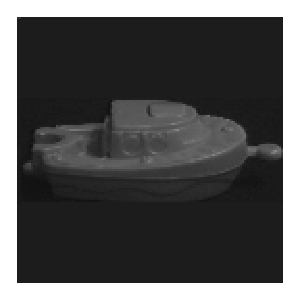
\includegraphics[width=2cm]{coil/beeld-27.eps} &
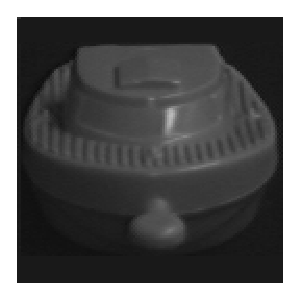
\includegraphics[width=2cm]{coil/beeld-28.eps} &
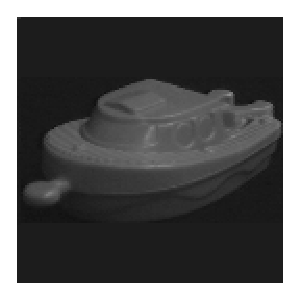
\includegraphics[width=2cm]{coil/beeld-29.eps} \\

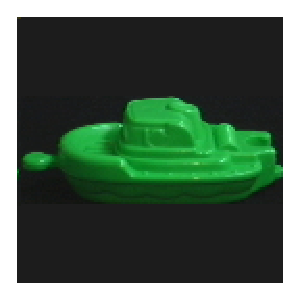
\includegraphics[width=2cm]{coil/beeld-54.eps} &
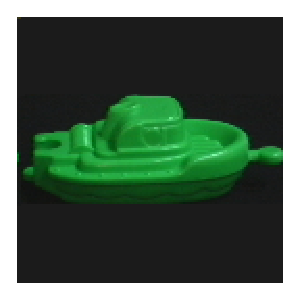
\includegraphics[width=2cm]{coil/beeld-55.eps} &
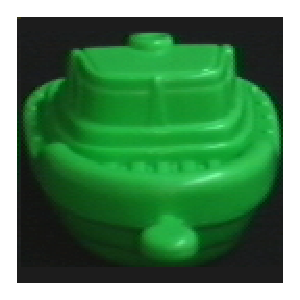
\includegraphics[width=2cm]{coil/beeld-56.eps} &
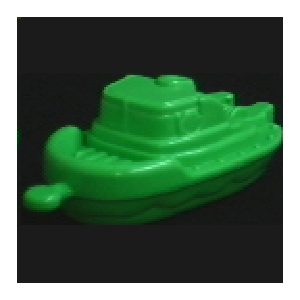
\includegraphics[width=2cm]{coil/beeld-57.eps} &
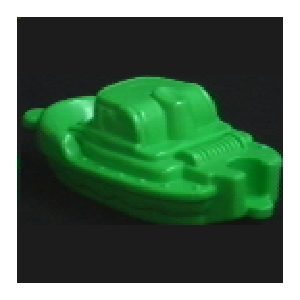
\includegraphics[width=2cm]{coil/beeld-58.eps} &
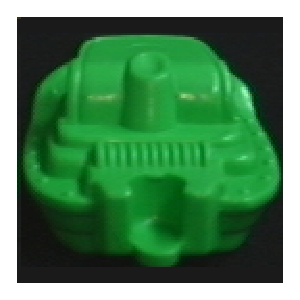
\includegraphics[width=2cm]{coil/beeld-59.eps} \\

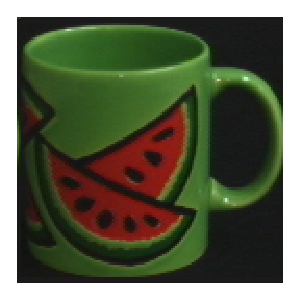
\includegraphics[width=2cm]{coil/beeld-30.eps} &
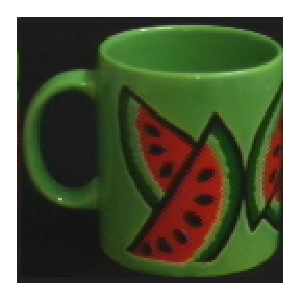
\includegraphics[width=2cm]{coil/beeld-31.eps} &
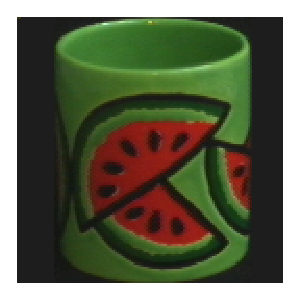
\includegraphics[width=2cm]{coil/beeld-32.eps} &
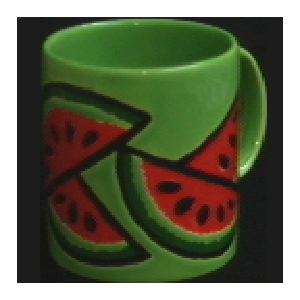
\includegraphics[width=2cm]{coil/beeld-33.eps} &
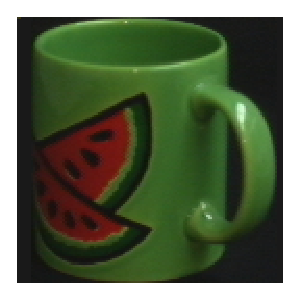
\includegraphics[width=2cm]{coil/beeld-34.eps} &
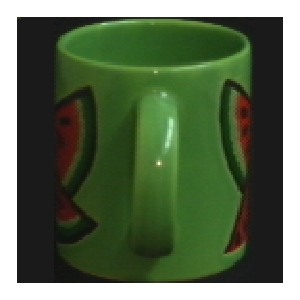
\includegraphics[width=2cm]{coil/beeld-35.eps} \\

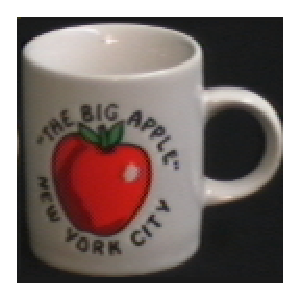
\includegraphics[width=2cm]{coil/beeld-36.eps} &
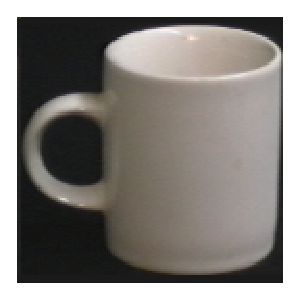
\includegraphics[width=2cm]{coil/beeld-37.eps} &
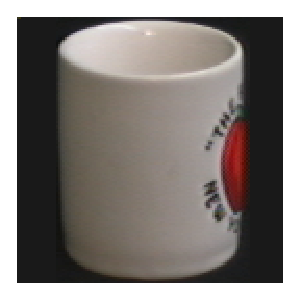
\includegraphics[width=2cm]{coil/beeld-38.eps} &
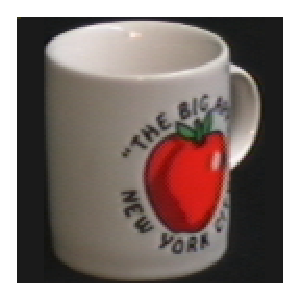
\includegraphics[width=2cm]{coil/beeld-39.eps} &
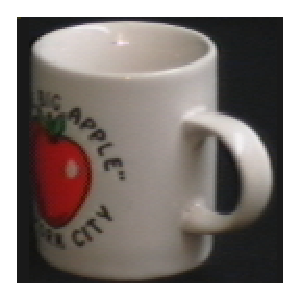
\includegraphics[width=2cm]{coil/beeld-40.eps} &
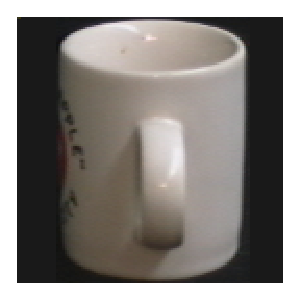
\includegraphics[width=2cm]{coil/beeld-41.eps} \\

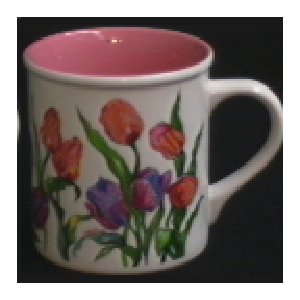
\includegraphics[width=2cm]{coil/beeld-6.eps} &
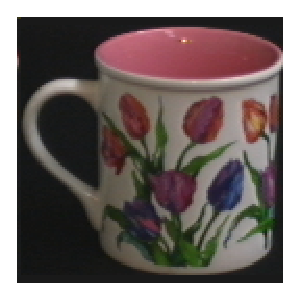
\includegraphics[width=2cm]{coil/beeld-7.eps} &
\includegraphics[width=2cm]{coil/beeld-8.eps} &
\includegraphics[width=2cm]{coil/beeld-9.eps} &
\includegraphics[width=2cm]{coil/beeld-10.eps} &
\includegraphics[width=2cm]{coil/beeld-11.eps} \\

\includegraphics[width=2cm]{coil/beeld-48.eps} &
\includegraphics[width=2cm]{coil/beeld-49.eps} &
\includegraphics[width=2cm]{coil/beeld-50.eps} &
\includegraphics[width=2cm]{coil/beeld-51.eps} &
\includegraphics[width=2cm]{coil/beeld-52.eps} &
\includegraphics[width=2cm]{coil/beeld-53.eps} \\

\includegraphics[width=2cm]{coil/beeld-60.eps} &
\includegraphics[width=2cm]{coil/beeld-61.eps} &
\includegraphics[width=2cm]{coil/beeld-62.eps} &
\includegraphics[width=2cm]{coil/beeld-63.eps} &
\includegraphics[width=2cm]{coil/beeld-64.eps} &
\includegraphics[width=2cm]{coil/beeld-65.eps} \\

\end{tabular}
\caption{\label{fig:testcollectie}De gebruikte collectie van afbeeldingen.}
\end{center}
\end{figure}

Voor het beoordelen van een rangschikking, gebruiken we de \emph{genormaliseerde gemiddelde rang} 
(GGR) \cite{muller:perf_eval}. Deze performantiemaat wordt toegepast op een collectie
van $N$ afbeeldingen. Voor elk van deze afbeeldingen bevat de collectie
$N_R$ zogenaamde \emph{relevante afbeeldingen}. In het geval van onze testcollectie geldt $N = 66$.
We gaan er in deze collectie vanuit dat foto's van eenzelfde object relevant zijn ten opzichte
van elkaar: $N_R = 6$. Beschouw nu de vector 
$(r_1,r_2,\ldots,r_{N_R}) \in \{1,2,\ldots,N\}^{N_R}$, waarbij $r_i$ het
rangnummer van de $i$-de relevante afbeelding voorstelt. De performantiemaat
wordt dan als volgt gedefinieerd:
\begin{definitie}
De genormaliseerde gemiddelde rang wordt gegeven door de volgende afbeelding:
$$
\begin{array}{lrcl}
\textrm{GGR}: 	& \{1,2,\ldots,N\}^{N_R} & \to 	& [0,1] \\
		& (r_1,r_2,\ldots,r_{N_R}) & \mapsto &
	{\displaystyle\frac{1}{N \cdot N_R}\left[ \left(\sum_{i=1}^{N_R}r_i\right) - \frac{N_R \cdot (N_R + 1)}{2} \right]},\\[15pt]
	& & & \qquad \quad \forall (r_1, r_2, ..., r_{N_R}) \in \{1,2,\ldots,N\}^{N_R}
\end{array}
$$
\end{definitie}
\noindent
Deze maat nadert naar 1 naarmate de performantie slechter wordt.

Tot nu toe hebben we er echter nog geen rekening mee gehouden dat de performantie van
een similariteitsmaat afhankelijk kan zijn van de gekozen voorbeeld-afbeelding. Dit probleem lossen we
op door de GGR te berekenen voor meerdere voorbeelden en het gemiddelde van de bekomen waarden
te beschouwen. We kiezen hierbij de beelden uit de linker kolom van 
figuur~\ref{fig:testcollectie} als voorbeeld-afbeeldingen. De waarde die we zo bekomen noemen we de
\emph{globale genormaliseerde gemiddelde rang} (GGGR). Het is deze waarde die we zullen gebruiken
om de performantie van een similariteitsmaat te evalueren. We zullen dus met andere woorden op
zoek gaan naar similariteitsmaten waarvan de GGGR zo klein mogelijk is.

\subsection{Rekentijd}

We zullen voor elke similariteitsmaat die we construeren ook meten hoelang het duurt om
de rangschikkingen, die nodig zijn om de GGGR te bepalen, te berekenen. Aan deze 
rekentijd hechten we echter niet zoveel belang als aan de GGGR, vermits het in onze
praktische implementatie niet absoluut noodzakelijk is dat de similariteitsmaten zo weinig
mogelijk rekentijd vereisen. De collecties van afbeeldingen waarop ze daar toegepast worden
zijn immers beperkt in grootte. Bovendien worden de berekeningen aan de kant van de client
uitgevoerd, waardoor er geen gevaar is voor overbelasting van de server.


\section{Pixel-gebaseerd}

\subsection{Grijswaardebeelden}

\subsubsection{Representatie}

Een \emph{binair beeld} is een beeld dat enkel witte en zwarte beeldpunten bevat. We kunnen een 
$n$-dimentionaal binair beeld dus modelleren als een scherpe verzameling $A$ in $\mathbb{R}^n$, met:
$$
\begin{array}{rcl}
x \in A & \iff & x \textrm{ is een wit punt in het beeld} \\
x \notin A & \iff & x \textrm{ is een zwart punt in het beeld}
\end{array}
$$ 
In de praktijk wordt een binair beeld echter voorgesteld als een rooster bestaande uit een
eindig aantal beeldpunten. Men kiest dus eerder $\mathbb{N}^2$ als universum.

Behalve wit en zwart, kan een \emph{grijswaardebeeld} ook grijstinten bevatten. Deze grijstinten
kunnen voorgesteld worden aan de hand van waarden uit het open eenheidsinterval $]0,1[$, waarbij
geldt: hoe groter de grijswaarde, hoe lichter de grijstint. Een $n$-dimensionaal grijswaardebeeld
kan dus gemodelleerd worden als een vaagverzameling $A$ in $\mathbb{R}^n$ bepaald door:
$$
\begin{array}{rcl}
A(x) = 1 & \iff & x \textrm{ is een wit punt in het beeld} \\
A(x) = 0 & \iff & x \textrm{ is een zwart punt in het beeld} \\
A(x) \in\ ]0,1[ & \iff & x \textrm{ is een beeldpunt met een grijstint}
\end{array}
$$
Ook bij grijswaardebeelden is het universum in de praktijk eerder $\mathbb{N}^2$.

\subsubsection{Similariteitsmaten}

Door de bovenstaande representatie te combineren met de vaagsimilariteitsmaten uit 
\ref{sectie:vaagsimilariteitsmaten}, bekomen we 23 similariteitsmaten. Deze maten
meten de gelijkenis tussen twee afbeeldingen door hun beeldpunten met elkaar te vergelijken.
Deze beeldpunten worden ook \emph{picture elements} of kortweg \emph{pixels} genoemd. Vandaar
dat we zeggen dat deze maten \emph{pixel-gebaseerd} zijn.

Men noemt het aantal pixels in een afbeelding de \emph{resolutie} van die afbeelding. Het is
duidelijk dat deze pixel-gebaseerde maten vereisen dat beide afbeeldingen dezelfde resolutie 
hebben.


\subsection{Kleurbeelden}
\label{sectie:pixelgeb_kleurbeelden}

\subsubsection{Kleurruimten}

Een \emph{kleurmodel} is een abstract mathematisch model dat beschrijft hoe kleuren gerepresenteerd 
kunnen worden als $n$-tallen. RGB is het meest gebruikte kleurmodel. In dit model is elke kleur
een gewogen som van drie hoofdkleuren: rood, groen en blauw. De gewichten van deze som
worden gebruikt als componenten van het drietal dat de kleur voorstelt. Naast RGB zijn ook
HSV en L*a*b* populaire kleurmodellen \cite{phillips:beeldverwerking}.

De kleuren die men op basis van een bepaald model kan voorstellen vormen een \emph{kleurruimte}. 
In het geval van RGB is dit een driedimensionale ruimte. De kleuren in deze ruimte zijn afhankelijk
van de manier waarop men ``rood'', ``groen'' en ``blauw'' definieert. Veelgebruikte kleurruimtes 
op basis van het RGB model zijn sRGB en Adobe RGB.

Hoewel het strikt gezien niet correct is, gebruikt men de term ``kleurruimte'' vaak ook voor het
kleurmodel. Men heeft het dus vaak over \emph{de} RGB kleurruimte, terwijl er eigenlijk meerdere
kleurruimtes bestaan die gebaseerd zijn op RGB. 

\subsubsection{Representatie}

In een \emph{kleurbeeld} heeft elke pixel een bepaalde kleur. Deze kleur wordt beschreven met
behulp van een kleurmodel. Ze wordt bijgevolg voorgesteld als een $n$-tal uit
$\mathbb{R}^n$. Dergelijke $n$-tallen kunnen we normaliseren tot $n$-tallen uit $[0,1]^n$. 

We beperken ons tot het RGB model en we beschouwen de ordening $\leq_{RGB,lex}$, die
gebaseerd is op de lexicografische ordening $\leq_{lex}$ en op de ordening voor kleuren in het 
RGB model uit \cite{dewitte:vect_morph_ops}:
$$
\begin{array}{rcl}
c <_{RGB} c' & \iff & d(c,Bl) < d(c',Bl)\ \lor \\
			   &	  & \quad(d(c,Bl) = d(c',Bl) \land d(c,Wh) > d(c',Wh)) \\[5pt]
c >_{RGB} c' & \iff & d(c,Wh) < d(c',Wh)\ \lor \\
			   &	  & \quad(d(c,Wh) = d(c',Wh) \land d(c,Bl) > d(c',Bl)) \\[5pt]
c =_{RGB} c'   & \iff & (d(c,Bl) = d(c',Bl) \land d(c,Wh) = d(c',Wh)) \\[10pt]
c \leq_{lex} c' & \iff & r < r' \lor (r = r' \land g < g') \lor (r = r' \land g = g' \land b < b') \\[10pt]
c \leq_{RGB,lex} c' & \iff & c <_{RGB} c' \lor (c =_{RGB} c' \land c \leq_{lex} c')
\end{array}
$$
waarbij $Bl = (0,0,0)$, $Wh = (1,1,1)$ en $d$ de Euclidische afstand.
Men kan gemakkelijk verifi\"eren dat $([0,1]^3,\leq_{RGB,lex})$ een complete tralie is, met:
$$
\begin{array}{@{}c@{}}
\begin{array}{rcrcll}
\inf \{c,c'\} & = & \min \{c,c'\} & = & c & \textrm{als } c <_{RGB} c' \\
		  	& & & = & c' & \textrm{als } c >_{RGB} c' \\
		  	& & & = & c & \textrm{als } c =_{RGB} c' \textrm{ en } c \leq_{lex} c' \\
		  	& & & = & c' & \textrm{anders} \\[10pt]
\sup \{c,c'\} & = & \max \{c,c'\} & = & c' & \textrm{als } c <_{RGB} c' \\
		  	& & & = & c & \textrm{als } c >_{RGB} c' \\
		  	& & & = & c' & \textrm{als } c =_{RGB} c' \textrm{ en } c \leq_{lex} c' \\
		  	& & & = & c & \textrm{anders}
\end{array}
\end{array}
$$
We kunnen een $m$-dimensionaal RGB-kleurbeeld dus modelleren als een L-vaagverzameling in 
$\mathbb{R}^m$, waarbij $L=[0,1]^3$. Net zoals bij grijswaardebeelden, is 
het universum in de praktijk echter eerder $\mathbb{N}^2$.

\subsubsection{Similariteitsmaten}

De klassieke manier om kleurbeelden te vergelijken gaat als volgt. Men past een similariteitsmaat 
voor grijswaardebeelden toe op elk van de kleurcomponenten en voegt daarna de resultaten van de
verschillende componenten samen. In het geval van het RGB model beschouwt men een
kleurbeeld dus als een combinatie van drie grijswaardebeelden. 

Een andere mogelijkheid is dat men het beeld eerst omzet naar een grijswaardebeeld, om er 
vervolgens een similariteitsmaat voor grijswaardebeelden op toe te passen. Deze omzetting kan 
bijvoorbeeld aan de hand van de formule $y = 0.3 \cdot r + 0.59 \cdot g + 0.11 \cdot b$ gebeuren.

In \ref{sectie:vaagsimilariteitsmaten} hebben echter vermeld dat de beschouwde 
vaagsimilariteitsmaten uitbreidbaar zijn naar L-vaag\-ver\-za\-me\-ling\-en met
$L=[0,1]^3$. Daarvoor moeten we de bewerkingen waarvan deze maten gebruik maken veralgemenen van 
$[0,1]$ naar $[0,1]^3$. 

Voor de vaagsimilariteitsmaten $M_1$ tot $M_3$ betekent dit concreet dat we een zinvolle betekenis 
moeten geven aan $c - c'$ en $|c|$, voor alle $c(r,g,b),c'(r',g',b') \in [0,1]^3$. We gebruiken
hiervoor 
$$
c - c' = (r-r',g-g',b-b') \quad \textrm{ en } \quad |c| = \frac{1}{\sqrt{3}} \cdot \sqrt{r^2 + g^2 + b^2}.
$$

Om de overige vaagsimilariteitsmaten te veralgemenen, hebben we een uitbreiding van het
begrip sigma count nodig. Hiervoor gebruiken we
$$
|A|=\frac{1}{\sqrt{n}}\sum_{x \in X}\sqrt{(A_1(x))^2+(A_2(x))^2+\ldots+(A_n(x))^2}
$$
met $n=3$. Deze overige maten maken bovendien ook gebruik van de bewerkingen $co$ (complement), 
$\cap$ (doorsnede) en $\cup$ (unie). Doordat we 
$(\mathcal{N},\mathcal{C},\mathcal{D})=(N_s,T_M,S_M)$ gekozen hebben, moeten we
dus $1 - c$, $\max \{c,c'\}$ en $\min \{c,c'\}$ kunnen bepalen voor alle 
$c(r,g,b),c'(r',g',b') \in [0,1]^3$. Hiervoor kunnen we $1 - c = (1,1,1) - (r,g,b)$ en de
bovenstaande definities gebruiken.

We kunnen kleurbeelden dus ook vergelijken door de bovenstaande representatie 
te combineren met (een veralgemeende versie van) \'e\'en van de 
vaagsimilariteitsmaten uit \ref{sectie:vaagsimilariteitsmaten}. 
Deze tralie-gebaseerde aanpak lijkt ons de meest interessante van de drie, omdat
de kleur-informatie hierbij het best behouden blijft.


\subsection{Resolutie-onafhankelijk}
\label{sectie:res-onafh}

Een belangrijke beperking van de bovenstaande pixel-gebaseerde similariteitsmaten is dat we
ze enkel kunnen toepassen op beelden die dezelfde resolutie hebben. We kunnen dit oplossen
door similariteitsmaten te construeren op een manier die ge\"inspireerd is op de constructie
van de zogenaamde omgeving-gebaseerde similariteitsmaten in \cite{vanderweken:similariteitsmaten}. 

Deze constructie gaat als volgt. Stel dat we twee afbeeldingen $A$ en $B$ willen
vergelijken. We verdelen
de te vergelijken afbeeldingen eerst in twee partities, die respectievelijk bestaan uit
$n$ en $m$ beeldonderdelen. Hierbij zorgen we ervoor dat de onderdelen
van deze beide partities allemaal dezelfde resolutie hebben. We kunnen deze onderdelen bijgevolg 
opvatten als kleine afbeeldingen, die men onderling kan vergelijken met behulp van de reeds 
geziene pixel-gebaseerde similariteitsmaten.

Vervolgens bepalen we de gemiddelde kleur van elk beeldonderdeel. Deze kleur gebruiken we om
de collecties van beeldonderdelen voor te stellen als twee geordende lijsten, op basis
van de ordening $\leq_{RGB,lex}$. De elementen van de lijst die correspondeert met $A$ noemen 
we $A_i$, $i \in \{1,2,\ldots,n\}$, en die van de andere lijst $B_j$, $j \in \{1,2,\ldots,m\}$.

Figuur~\ref{fig:multires} illustreert de constructie van deze lijsten voor twee concrete
kleurbeelden. In deze figuur is de kleur van een beeldonderdeel gelijk aan de gemiddelde 
kleur van dat onderdeel.
\begin{figure}[tbp]
\begin{center}
\includegraphics[width=\textwidth]{images/multires.eps}
\caption{\label{fig:multires}Constructie van een resolutie-onafhankelijke similariteitsmaat op basis van een pixel-gebaseerde maat.}
\end{center}
\end{figure}
\begin{table}
\begin{center}
\begin{tabular}{|c|ccccccccc|}
\hline
$\scriptstyle M_3(A_i,B_j)$	& $B_1$ & $B_2$ & $B_3$ & $B_4$ & $B_5$ & $B_6$ & $B_7$ & $B_8$ & $B_9$  \\
\hline
$A_1$ 	& $\mathbf{\scriptstyle 0.5198}$ & $\scriptstyle 0.4496$ & & & & & & & \\
$A_2$ 	& & $\mathbf{\scriptstyle 0.4691}$ & $\scriptstyle 0.3859$ & & & & & & \\
$A_3$ 	& & & $\scriptstyle 0.4133$ & $\mathbf{\scriptstyle 0.4404}$ & $\scriptstyle 0.3298$ & & & & \\
$A_4$ 	& & & & & $\scriptstyle 0.3277$ & $\mathbf{\scriptstyle 0.4330}$ & $\scriptstyle 0.3648$ & & \\
$A_5$ 	& & & & & & & $\mathbf{\scriptstyle 0.3849}$ & $\scriptstyle 0.3134$ & \\
$A_6$ 	& & & & & & & & $\mathbf{\scriptstyle 0.3438}$ & $\scriptstyle 0.3427$ \\
$A_7$ 	& & & & & & & & & $\mathbf{\scriptstyle 0.5066}$ \\
\hline
\end{tabular}
\caption{\label{tab:multires}De similariteiten die berekend worden in de constructie die ge\"illustreerd wordt door figuur~\ref{fig:multires}.}
\end{center}
\end{table}

Zodra we beschikken over de twee geordende lijsten, overlopen we de elementen van de 
lijst die correspondeert met $B$. Voor
elk element dat we tegenkomen, bepalen we de similariteit met $A_1$. Dit blijven we doen
tot we een similariteit vinden die kleiner is dan de vorige. We stoppen dus na $i$ iteraties 
indien $A_1$ en $B_i$ minder gelijkenis vertonen dan $A_1$ en $B_{i-1}$. Op dat moment voegen
we de similariteit tussen $A_1$ en $B_{i-1}$ toe aan de lijst van similariteiten $S$. Daarna
beginnen we bij $B_i$ en herhalen we deze procedure voor $A_2$. We voegen dus opnieuw de vorige
similariteit toe aan $S$ als deze groter is dan de huidige. Zo gaan we verder tot we bij
$B_m$ komen. Als we deze procedure $j$ keer kunnen herhalen, dan
is de similariteit tussen $A_j$ en $B_m$ dus de laatste die we berekenen. Deze similariteit
voegen we ook nog toe aan $S$. Tenslotte bepalen we de globale similarteit tussen $A$ en $B$ 
door het gemiddelde van de waarden uit $S$ te berekenen.

Tabel~\ref{tab:multires} geeft een overzicht van de 
verschillende similariteiten die berekend worden indien we de bovenstaande constructie
toepassen op de kleurbeelden uit figuur~\ref{fig:multires}. We hebben hierbij gebruik gemaakt 
van de vaagsimilariteitsmaat $M_3$ en de tralie-gebaseerde aanpak uit \ref{sectie:pixelgeb_kleurbeelden}.
De similariteiten die  
toegevoegd worden aan $S$ staan in het vet. Deze similariteiten 
worden in figuur~\ref{fig:multires} grafisch weergeven als verbindingen tussen de
geordende beeldonderdelen.

De constructie van een resolutie-onafhankelijke similariteitsmaat, 
op basis van een pixel-gebaseerde maat, bestaat dus uit vier stappen:
\begin{enumerate}
\item Verdeel de te vergelijken afbeeldingen $A$ en $B$
in partities, zodanig dat alle beeldonderdelen dezelfde resolutie hebben.
\item Bepaal de gemiddelde kleur van elk beeldonderdeel. Gebruik deze kleur vervolgens
om de beide collecties van beeldonderdelen te ordenen met behulp van de ordening $\leq_{RGB,lex}$.
\item Overloop de beeldonderdelen van $B$ en bepaal telkens de similariteit met het eerste 
beeldonderdeel van $A$. Voeg de vorige similariteit toe aan de lijst van similariteiten $S$
indien ze groter is dan de huidige. Herhaal deze stap op dat moment voor de resterende
beeldonderdelen van $A$ en $B$. Het 
beeldonderdeel van $B$ dat aanleiding gaf tot de huidige similariteit maakt deel uit van
deze resterende beeldonderdelen.

Als het laatste beeldonderdeel van $B$ bereikt wordt, dan wordt de similariteit tussen dit
beeldonderdeel en het huidige beeldonderdeel van $A$ toegevoegd aan $S$. De overblijvende
beeldonderdelen van $A$ worden dan buiten beschouwing gelaten. 
\item Bepaal het gemiddelde van de similariteiten uit $S$. Deze waarde is de globale similariteit tussen
$A$ en $B$.
\end{enumerate}

Het resultaat $M$ van deze constructie, voor twee beelden $A$ en $B$, is echter niet noodzakelijk 
een symmetrische similariteitsmaat. Om dit probleem op te lossen, bepalen we zowel $M(A,B)$ als
$M(B,A)$ en gebruiken we het gemiddelde van deze waarden.


\subsection{Experimentele observaties}

\begin{figure}[tbp]
\begin{center}
\includegraphics[width=\textwidth]{plots/pixelgeb_gggrs_en_cputimes_filled.eps}
\caption{\label{fig:pixelgeb_gggrs_en_cputimes}De GGGR-waarde en de gebruikte rekentijd in ms voor elk van de resolutie-onafhankelijke pixel-gebaseerde similariteitsmaten.}
\end{center}
\end{figure}

In figuur~\ref{fig:pixelgeb_gggrs_en_cputimes} vergelijken we enkele pixel-gebaseerde similariteitsmaten.
Hoewel de afbeeldingen in onze testcollectie allemaal dezelfde resolutie hebben, zullen de
resoluties van de beelden die we in de praktijk gaan vergelijken vrijwel altijd verschillend zijn.
We beperken ons daarom tot resolutie-onafhankelijke similariteitsmaten. Deze maten construeren
we op basis van een pixel-gebaseerde maat, zoals besproken in \ref{sectie:res-onafh}. De 
beeldonderdelen die we gebruiken bestaan uit $8 \cdot 8 = 64$ pixels.

We beschouwen de drie bovenstaande manieren om de vaagsimilariteitsmaten toe te passen op een 
onderdeel van een kleurbeeld:
eerst omzetten naar een grijswaardebeeld, 
toepassen op de afzonderlijke kleurcomponenten en 
de tralie-gebaseerde aanpak.
De laatste manier in combinatie met $M_{3}$ levert de beste similariteitsmaat op. We vinden
voor deze similariteitsmaat de GGGR-waarde $0.16255411255411253$. Dit is echter nog steeds een
vrij hoge waarde. In figuur~\ref{fig:results_beste_pixelgeb}
zien we dan ook dat de resultaten van deze maat niet zo overtuigend zijn. Blijkbaar 
is de pixel-gebaseerde benadering niet de meest geschikte voor image retrieval. 

\begin{figure}[tbp]
\begin{center}
\begin{tabular}{m{11cm} | m{3cm} |}
\textbf{Eerste tien resultaten:} & \textbf{GGR:} \\
\vspace{4pt}
\includegraphics[width=1cm]{coil/beeld-18.eps}
\includegraphics[width=1cm]{coil/beeld-22.eps}
\includegraphics[width=1cm]{coil/beeld-20.eps}
\includegraphics[width=1cm]{coil/beeld-19.eps}
\includegraphics[width=1cm]{coil/beeld-18.eps}
\includegraphics[width=1cm]{coil/beeld-3.eps}
\includegraphics[width=1cm]{coil/beeld-21.eps}
\includegraphics[width=1cm]{coil/beeld-7.eps}
\includegraphics[width=1cm]{coil/beeld-43.eps}
\includegraphics[width=1cm]{coil/beeld-12.eps}
& {\scriptsize 0.002380952380952381}
\\
\includegraphics[width=1cm]{coil/beeld-24.eps}
\includegraphics[width=1cm]{coil/beeld-26.eps}
\includegraphics[width=1cm]{coil/beeld-28.eps}
\includegraphics[width=1cm]{coil/beeld-25.eps}
\includegraphics[width=1cm]{coil/beeld-48.eps}
\includegraphics[width=1cm]{coil/beeld-51.eps}
\includegraphics[width=1cm]{coil/beeld-24.eps}
\includegraphics[width=1cm]{coil/beeld-49.eps}
\includegraphics[width=1cm]{coil/beeld-27.eps}
\includegraphics[width=1cm]{coil/beeld-48.eps}
& {\scriptsize 0.011904761904761904}
\\
\includegraphics[width=1cm]{coil/beeld-60.eps}
\includegraphics[width=1cm]{coil/beeld-63.eps}
\includegraphics[width=1cm]{coil/beeld-60.eps}
\includegraphics[width=1cm]{coil/beeld-61.eps}
\includegraphics[width=1cm]{coil/beeld-30.eps}
\includegraphics[width=1cm]{coil/beeld-33.eps}
\includegraphics[width=1cm]{coil/beeld-54.eps}
\includegraphics[width=1cm]{coil/beeld-64.eps}
\includegraphics[width=1cm]{coil/beeld-57.eps}
\includegraphics[width=1cm]{coil/beeld-31.eps}
& {\scriptsize 0.05}
\\
\includegraphics[width=1cm]{coil/beeld-48.eps}
\includegraphics[width=1cm]{coil/beeld-26.eps}
\includegraphics[width=1cm]{coil/beeld-28.eps}
\includegraphics[width=1cm]{coil/beeld-24.eps}
\includegraphics[width=1cm]{coil/beeld-25.eps}
\includegraphics[width=1cm]{coil/beeld-27.eps}
\includegraphics[width=1cm]{coil/beeld-51.eps}
\includegraphics[width=1cm]{coil/beeld-24.eps}
\includegraphics[width=1cm]{coil/beeld-49.eps}
\includegraphics[width=1cm]{coil/beeld-48.eps}
& {\scriptsize 0.06904761904761905}
\\
\includegraphics[width=1cm]{coil/beeld-54.eps}
\includegraphics[width=1cm]{coil/beeld-58.eps}
\includegraphics[width=1cm]{coil/beeld-31.eps}
\includegraphics[width=1cm]{coil/beeld-56.eps}
\includegraphics[width=1cm]{coil/beeld-33.eps}
\includegraphics[width=1cm]{coil/beeld-30.eps}
\includegraphics[width=1cm]{coil/beeld-32.eps}
\includegraphics[width=1cm]{coil/beeld-1.eps}
\includegraphics[width=1cm]{coil/beeld-30.eps}
\includegraphics[width=1cm]{coil/beeld-60.eps}
& {\scriptsize 0.10238095238095238}
\\
\includegraphics[width=1cm]{coil/beeld-12.eps}
\includegraphics[width=1cm]{coil/beeld-12.eps}
\includegraphics[width=1cm]{coil/beeld-14.eps}
\includegraphics[width=1cm]{coil/beeld-0.eps}
\includegraphics[width=1cm]{coil/beeld-3.eps}
\includegraphics[width=1cm]{coil/beeld-0.eps}
\includegraphics[width=1cm]{coil/beeld-42.eps}
\includegraphics[width=1cm]{coil/beeld-43.eps}
\includegraphics[width=1cm]{coil/beeld-22.eps}
\includegraphics[width=1cm]{coil/beeld-1.eps}
& {\scriptsize 0.10952380952380952}
\\
\includegraphics[width=1cm]{coil/beeld-30.eps}
\includegraphics[width=1cm]{coil/beeld-60.eps}
\includegraphics[width=1cm]{coil/beeld-63.eps}
\includegraphics[width=1cm]{coil/beeld-60.eps}
\includegraphics[width=1cm]{coil/beeld-33.eps}
\includegraphics[width=1cm]{coil/beeld-61.eps}
\includegraphics[width=1cm]{coil/beeld-31.eps}
\includegraphics[width=1cm]{coil/beeld-1.eps}
\includegraphics[width=1cm]{coil/beeld-64.eps}
\includegraphics[width=1cm]{coil/beeld-3.eps}
& {\scriptsize 0.11904761904761904}
\\
\includegraphics[width=1cm]{coil/beeld-6.eps}
\includegraphics[width=1cm]{coil/beeld-60.eps}
\includegraphics[width=1cm]{coil/beeld-63.eps}
\includegraphics[width=1cm]{coil/beeld-60.eps}
\includegraphics[width=1cm]{coil/beeld-61.eps}
\includegraphics[width=1cm]{coil/beeld-1.eps}
\includegraphics[width=1cm]{coil/beeld-64.eps}
\includegraphics[width=1cm]{coil/beeld-3.eps}
\includegraphics[width=1cm]{coil/beeld-30.eps}
\includegraphics[width=1cm]{coil/beeld-43.eps}
& {\scriptsize 0.26904761904761904}
\\
\includegraphics[width=1cm]{coil/beeld-0.eps}
\includegraphics[width=1cm]{coil/beeld-60.eps}
\includegraphics[width=1cm]{coil/beeld-61.eps}
\includegraphics[width=1cm]{coil/beeld-63.eps}
\includegraphics[width=1cm]{coil/beeld-60.eps}
\includegraphics[width=1cm]{coil/beeld-45.eps}
\includegraphics[width=1cm]{coil/beeld-30.eps}
\includegraphics[width=1cm]{coil/beeld-42.eps}
\includegraphics[width=1cm]{coil/beeld-3.eps}
\includegraphics[width=1cm]{coil/beeld-1.eps}
& {\scriptsize 0.33095238095238094}
\\
\includegraphics[width=1cm]{coil/beeld-42.eps}
\includegraphics[width=1cm]{coil/beeld-60.eps}
\includegraphics[width=1cm]{coil/beeld-61.eps}
\includegraphics[width=1cm]{coil/beeld-45.eps}
\includegraphics[width=1cm]{coil/beeld-0.eps}
\includegraphics[width=1cm]{coil/beeld-63.eps}
\includegraphics[width=1cm]{coil/beeld-60.eps}
\includegraphics[width=1cm]{coil/beeld-33.eps}
\includegraphics[width=1cm]{coil/beeld-30.eps}
\includegraphics[width=1cm]{coil/beeld-1.eps}
& {\scriptsize 0.33095238095238094}
\\
\includegraphics[width=1cm]{coil/beeld-36.eps}
\includegraphics[width=1cm]{coil/beeld-60.eps}
\includegraphics[width=1cm]{coil/beeld-61.eps}
\includegraphics[width=1cm]{coil/beeld-63.eps}
\includegraphics[width=1cm]{coil/beeld-60.eps}
\includegraphics[width=1cm]{coil/beeld-1.eps}
\includegraphics[width=1cm]{coil/beeld-3.eps}
\includegraphics[width=1cm]{coil/beeld-45.eps}
\includegraphics[width=1cm]{coil/beeld-0.eps}
\includegraphics[width=1cm]{coil/beeld-64.eps}
& {\scriptsize 0.39285714285714285}
\end{tabular}
\caption{\label{fig:results_beste_pixelgeb}De GGR-waarde en de eerste tien resultaten voor elke voorbeeld-afbeelding bij de beste resolutie-onafhankelijke pixel-gebaseerde similariteitsmaat.}
\end{center}
\end{figure}

Op het vlak van rekentijd zijn de similariteitsmaten op basis van de eerste en de laatste manier
aan elkaar gewaagd. Bij het toepassen van een similariteitsmaat voor grijswaardebeelden op de 
afzonderlijke kleurcomponenten, hebben we echter aanzienlijk meer rekentijd nodig. Dit is niet
verwonderlijk, vermits er dan ook driemaal zoveel werk moet verricht worden.


\section{Histogram-gebaseerd}

Kleur is \'e\'en van de meest gebruikte kenmerken bij CBIR. Het kleurhistogram is de meest 
populaire representatie van dit kenmerk \cite{rui:image_retr}. We mogen dus verwachten
dat deze histogrammen kunnen gebruikt worden om effici\"ente similariteitsmaten te construeren.
In deze sectie onderzoeken we of dit effectief het geval is. 

Een histogram van een kleurbeeld is een voorstelling van de frequentieverdeling van de
verschillende kleuren. De waarde van het histogram voor een kleurbeeld $A$ in de kleur $c$ is
dus gelijk aan het totaal aantal pixels in het beeld met kleur $c$. We noteren dit met $h_A(c)$:
$$
h_A(c) = \sum_{x \in X} \delta (c - A(x))
$$
waarbij $\delta$ de Diracfuntie is en $X$ het universum der beelpunten voorstelt. 


\subsection{Pseudo-vage histogrammen}

Door de waarden van een histogram te normaliseren, kunnen we het omzetten naar een 
vaagverzameling in $C$, waarbij $C$ het universum der kleuren is. Dit houdt in dat we elke
waarde van het histogram delen door het maximaal aantal pixels met dezelfde kleur. 
We hebben dus de volgende uitdrukking voor de lidmaatschapsgraad van de kleur $c$ in de 
vaagverzameling $PFh_A$ geassocieerd met het histogram van beeld $A$:
$$
PFh_A(c) = \frac{\displaystyle h_A(c)}{\displaystyle \max_{c \in C}(c)}
$$

Voor een RGB-beeld gebruikt men typisch 8 bits per kleurcomponent. Dit geeft een totaal van
24 bits per kleur, zodat men dus $2^{24}=2^4 \cdot 2^{20}=16 \cdot 2^{20} \approx 16 \cdot 10^6$
kleuren kan voorstellen. Een genormaliseerd histogram bestaat dan dus uit 16 miljoen waarden.
Similariteitsmaten op basis van dergelijke histogrammen zouden dus veel te veel rekentijd vragen.

We kunnen de rekentijd echter reduceren door de histogrammen te comprimeren. Dit kan 
gerealiseerd worden door gebruik te 
maken van zogenaamde \emph{bins}. Elk van deze bins omvat meerdere kleuren. We beschouwen dus 
geen aparte kleuren meer, maar wel verzamelingen van kleuren. Per verzameling bepalen we dan 
hoeveel keer de kleuren in die verzameling voorkomen 
in de afbeelding in kwestie. De karakteristieke afbeelding van de vaagverzameling $BPFh_A$, die
correspondeert met het in $N$ bins onderverdeelde histogram van beeld $A$, wordt dan als volgt
gedefinieerd:  
$$
\begin{array}{lrcl}
BPFh_A: 	& \{1,2,\ldots,N\} 	& \to 		& [0,1] \\[5pt]
		& n						& \mapsto	& \displaystyle\sum_{c \in C} \delta (n -  bin(c)),
\quad\forall n \in \{1,2,\ldots,N\}
\end{array}
$$
Hierbij is $bin$ een $C - \{1,2,\ldots,N\}$ afbeelding die met elke kleur het nummer van de 
corresponderende bin associeert. We zouden bijvoorbeeld 
$bin(c) = \lfloor PFh_A(c) \cdot (N-1) \rfloor + 1$ kunnen kiezen. Doorgaands willen we echter
meer belang hechten aan bepaalde kleurcomponenten. We gebruiken daarom de volgende definitie:
$$
bin(c) = bin(c_1,c_2,\ldots,c_m) = \left[ \sum_{i=1}^m \left( \prod_{j=1}^{i-1} N_j \right) \left\lfloor c_i \cdot (N_i - 1) \right\rfloor \right] + 1
$$
met $N=N_1 \cdot N_2 \cdot \ldots \cdot N_m$.

\subsubsection{HSV-histogram}

In het HSV kleurmodel wordt elke kleur voorgesteld door een drietal. Men noemt de componenten van 
zo'n drietal respectievelijk ``hue'', ``saturation'' en ``value''. De eerste van deze componenten
correspondeert met de kleurtint, terwijl de overige componenten de verzadiging en de helderheid
aangeven. Men kan een kleur $c(r,g,b) \in [0,1]^3$ uit het RGB model als volgt omzetten naar een 
kleur $c'(h,s,v) \in [0,1]^3$ in het HSV model:
$$
\begin{array}{rcll}
h' & = & 60 \cdot \frac{g - b}{\max \{r,g,b\} - \min \{r,g,b)}\quad & \textrm{ als } \max \{r,g,b\} = r \\[2pt]
  & = & 60 \cdot \frac{b - r}{\max \{r,g,b\} - \min \{r,g,b)} + 120\quad & \textrm{ als } \max \{r,g,b\} = g \\[2pt]
  & = & 60 \cdot \frac{r - g}{\max \{r,g,b\} - \min \{r,g,b)} + 240\quad & \textrm{ als } \max \{r,g,b\} = b \\[6pt]
h & = & \frac{h' \bmod 360}{360} & \textrm{ als } h' \bmod 360 \geq 0 \\[2pt]
  & = & \frac{360 - (h' \bmod 360)}{360} & \textrm{ als } h' \bmod 360 < 0 \\[6pt]
s & = & \frac{\max \{r,g,b\} - \min \{r,g,b\}}{\max \{r,g,b\}} & \\[6pt]
v & = & \max \{r,g,b\}
\end{array}
$$
Als $s=0$ dan is $h$ niet gedefinieerd. Dit is logisch vermits we dan te maken hebben met een 
grijswaarde. Indien $v=0$ dan is $s$ niet gedefinieerd. We hebben het in dat geval dan ook over 
puur zwart, waarvoor er geen kleurtint of saturatie kan gespecifieerd worden. In de praktische
implementatie geven we niet gedefinieerde componenten de waarde 0.

Bij image retrieval is doorgaands vooral de kleurtint op zich belangrijk. We kunnen de grootte van
een histogram dus beperken door het HSV model te gebruiken en meer belang te hechten aan de
eerste kleurcomponent. Dit doen we door $N_1=16$, $N_2=4$ en $N_3=4$ te kiezen. We bekomen zo dus
een histogram dat slechts $16 \cdot 4 \cdot 4 = 256$ waarden bevat. 
%Bovendien is het discriminerend
%vermogen van dit histogram waarschijnlijk ook beter dan dat van een ongecomprimeerd kleurhistogram.

Merk op dat onze keuzes voor $N_1$, $N_2$ en $N_3$ overeenstemmen met de keuzes die men gemaakt
heeft voor de \emph{scalable color descriptor} (SCD), die gedefinieerd wordt in de MPEG-7
standaard \cite{manjunath:color_and_texture_descriptors}.

\subsubsection{OCS-histogram}

\subsubsection{HMMD-histogram}

\subsubsection{NCS-histogram}

\subsubsection{XYZ-histogram}

\subsubsection{Yxy-histogram}


\subsubsection{Experimentele observaties}


\subsection{Vaaghistogram}

Naast de bovenstaande vage interpretatie van het klassieke kleurhistogram, beschouwen we
ook nog een kleurbeschrijving die we op een ``volledig vage'' manier opbouwen. Bij dit
\emph{vaaghistogram} maken we gebruik van het L*a*b* kleurmodel en beschouwen we een 
vaagverzameling voor elke kleur. 
De lidmaatschapsgraad van een kleur $c'$ in de vaagverzameling 
$FC_c$, die correspondeert met kleur $c$, defini\"eren we als volgt \cite{vertan:fuzzy_histograms}: 
$$
\begin{array}{rcll}
FC_c(c') & = & 1 & \textrm{als } d(c,c') \leq 2.3 \\
		 & = & \exp \left( - \frac{\left((d(c,c') / 2.3) - 1\right)^2}{2 \cdot \lambda^2} \right) & \textrm{anders}
\end{array}
$$  
met $d$ de Euclidische afstand en $\lambda$ een vrij te kiezen parameter, die we in deze scriptie
voor de eenvoud steeds gelijk aan $1$ zullen kiezen. In het geval van L*a*b* 
komt de afstand $2.3$ namelijk overeen met de zogenaamde \emph{just noticeable difference} (JND)
\cite{sharma:digital_color_imaging}. 
Kleuren waarvan de onderlinge afstand kleiner dan of gelijk aan deze JND is, kunnen door de mens 
niet onderscheiden worden.

Het eigenlijk vaaghistogram $Fh_A$, voor een kleurbeeld $A$, defini\"eren we dan als de unie van 
alle kleuren die voorkomen in $A$:
$$
Fh_A = \displaystyle\bigcup_{c \in C_A} FC_c
%\begin{array}{lrcl}
%Fh_A: 	& C_A 	& \to 		& [0,1] \\[5pt]
%		& c					& \mapsto	& \displaystyle\bigcup_{c \in C_A} FC_c,
%\quad\forall c \in C_A
%\end{array}
$$ 
waarbij de verzameling $C_A$ bestaat uit de in $A$ voorkomende kleuren.

\subsubsection{Experimentele observaties}


\section{Gebaseerd op dominante kleuren}
